%% LyX 2.3.4.2 created this file.  For more info, see http://www.lyx.org/.
%% Do not edit unless you really know what you are doing.
\documentclass[twoside,english]{elsarticle}
\usepackage[T1]{fontenc}
\usepackage[latin9]{inputenc}
\pagestyle{headings}
\usepackage{float}
\usepackage{amsmath}
\usepackage{graphicx}

\makeatletter

%%%%%%%%%%%%%%%%%%%%%%%%%%%%%% LyX specific LaTeX commands.
%% Because html converters don't know tabularnewline
\providecommand{\tabularnewline}{\\}

%%%%%%%%%%%%%%%%%%%%%%%%%%%%%% User specified LaTeX commands.
% specify here the journal
\journal{Engineering Applications of Artificial Intelligence}

% use this if you need line numbers
%\usepackage{lineno}

\@ifundefined{showcaptionsetup}{}{%
 \PassOptionsToPackage{caption=false}{subfig}}
\usepackage{subfig}
\makeatother

\usepackage{babel}
\begin{document}

\begin{frontmatter}{}

\title{DIGITAL ROCK CHARACTERIZATION USING ARTIFICIAL INTELLIGENCE - APPLICATION
TO IMAGE SEGMENTATION}

\author[lenep]{J.~M.~C.~Carvalho\fnref{fn1}}

\ead{joao.carvalho@lenep.uenf.br}

\author[lenep]{A.~D.~Bueno\fnref{fn2}}

\ead{bueno@lenep.uenf.br}

\address[lenep]{Av. Alberto Lamego, 2000 \textendash{} Parque Calif�rnia \textendash{}
Campos dos Goytacazes \textendash{} RJ - Brazil \textendash{} CEP:
28013-602}
\begin{abstract}
In the field of digital rock segmentation, the use of neural networks
allows the classification or determination of solid and porous phases.
The purpose of this work was to show how the use of such methods makes
the binarization of images of reservoir rocks in solids and pores
practical. For this, the color information of an image, collected
through an annotation software developed in C++. The construction
and training of neural networks were made with the PyTorch library
through python scripts. Each training sequence (loading the dataset,
separating it into training and test sets, and then into mini-batches,
performing batch training and testing the result in each epoch) lasted
about 12 milliseconds. The results were obtained with an error varying
between 6\% and 80\% in comparison with laboratory measurements. It
is believed that this occurs due to the points obtained from the regions
of interest in the image, so a more careful collection could guarantee
better results. 
\end{abstract}
\begin{keyword}
Artificial Intelligence \sep Digital Rock \sep Neural Networks
\end{keyword}

\end{frontmatter}{}

\section{Introduction}

In this work, a study is developed about the application of artificial
intelligence algorithms in the processing of images of reservoir rocks.
More specifically, it is focused on the process of binarization of
them, in order to facilitate the characterization of petrophysical
properties.

\subsection{Description of the Problem}

It is increasingly common to apply artificial intelligence algorithms
in the most different areas of research, especially in engineering.
The use of intelligent algorithms makes it possible to perform complex
classification and prediction tasks in a short time. Methods of such
nature had been predicted for decades, but only with the exponential
increase in the processing capacity of computers and the decrease
in their cost has made then possible.

Recent advances in the field of imaging technology make rock analysis
through digital imaging emergent. Microtomographs allow a non-destructive
analysis of cores and help to build a more complete understanding
of physical processes in porous media.

As shown in the work of \citet{andra2013digital,rubo2019digital}
the choice of a segmentation algorithm, filters and especially the
threshold in gray-scale images are the key points for a good binarization
of a reservoir rock image sample, so much that an unfortunate combination
of these parameters can bring ambiguities for the interpretation process.

\citet{rego2010desenvolvimento} showed that the use of artificial
neural networks can bring good results to the image segmentation process,
especially when compared to traditional methods. However, it is worth
noting that there was still a difficulty in processing samples in
which very light or dark grains were found. In addition, the work
used traditional feed-forward neural networks, backpropagation algorithm,
quadratic cost function and sigmoid activation function.

With the advancement of AI methods these choices have become obsolete
over the years, and works like those of \citet{sudakov2019driving,rubo2019digital,van2016machine,saporetti2018machine}
has been showing good results on the processing of what can be called
Digital Rock using, for example, convolutional neural networks combined
with simpler machine learning algorithms.

These factors therefore contribute to the motivation of this work,
which aims to use the experience obtained in previous works to advance
knowledge in the field of research in Artificial Intelligence applied
to petroleum reservoir engineering.

\subsection{Artificial Neural Networks}

Artificial neural networks are defined as non-linear models capable
of mimicking the behavior of the human brain and its neuron structure
\citep{haykin2007redes}. Thus, ideally, an ANN is capable of performing
the operations of learning, association, generalization and abstraction.
These networks are composed of a series of elements called artificial
neurons, highly interconnected and that perform simple operations
and pass the information to the following elements of the structure.
Each entry is represented by $u_{i}$ and is weighted by a weight
$w_{i}$ with i ranging from $1$ to $n$. The combination of these
inputs is done by the sum $\Phi$, to which a value of polarization
or bias $\theta$ is added, as shown in Equation \ref{eq:weighted-sum}.

\begin{equation}
u=\Phi+\theta=\sum_{1}^{n}u_{n}w_{n}+\theta\label{eq:weighted-sum}
\end{equation}

The result of the operation shown in Equation \ref{eq:weighted-sum}
is applied as input to an activation function $\eta$, thus the output
$y$ of the neuron is shown in Equation \ref{eq:neuron-output}. This
activation function that is responsible for introducing non-linearity
to the neuron model, and can appear in the form of a hyperbolic tangent,
sigmoid function, \emph{ReLU}, among others \citep{chollet2018deep}.

\begin{equation}
y=\eta(u)=\eta\left(\Phi+\theta\right)=\eta\left(\sum_{1}^{n}u_{n}w_{n}+\theta\right)\label{eq:neuron-output}
\end{equation}

The ReLU activation function shown in Equation \ref{eq:relu-func}
has as its main advantage the fact that it does not immediately activate
all neurons, as negative values of u end up being set to $0$ \citep{nielsen2015neural}.

\begin{equation}
\eta(u)=\begin{cases}
u & u\geq0\\
0 & u<0
\end{cases}\label{eq:relu-func}
\end{equation}

The softmax function is similar to a sigmoid function and is widely
used for classifying problems with more than two classes. It converts
the values of the output layers into a probability function. Equation
\ref{eq:softmax-func} shows its structure, where $\vec{u}$ represents
an entire input vector with k elements $u_{i}$. Here $k$ is also
the number of classes applied to the algorithm.

\begin{equation}
\eta(\vec{u})_{i}=\frac{e^{u_{i}}}{\sum_{j=1}^{k}e^{u_{j}}}\label{eq:softmax-func}
\end{equation}


\subsection{Feed-forward Neural Networks}

\citet{nielsen2015neural} defines feed-forward neural networks as
structures divided in layers that are always fed with data in one
direction. Any layer between these two is called deep or hidden layers. 

The behavior of this neural network can be expressed in the form of
Equation \ref{eq:rna-direct-notation}. In this notation $w_{jk}^{l}$
denotes the weight of the connection between the $k$-th neuron of
the $(l-1)$-th layer with the $j$-th neuron of the $l$-th layer.
Furthermore$\theta_{j}^{l}$ and $y_{j}^{l}$ represent, respectively,
the bias and activation of the $j$-th neuron in the $l$-th layer.
The activation of the $k$-th neuron of the previous layer ($l-1$)
is used as input for the activation of the current neuron and is represented
as $y_{k}^{l-1}$. Equation \ref{eq:vetorized-form} shows the vectorized
form of the activation.

\begin{equation}
y_{j}^{l}=\eta\left(\sum_{k}w_{jk}^{l}y_{k}^{l-1}+\theta_{j}^{l}\right)\label{eq:rna-direct-notation}
\end{equation}

\begin{equation}
y^{l}=\eta\left(w^{l}y^{l-1}+\theta^{l}\right)\label{eq:vetorized-form}
\end{equation}

According with \citet{goodfellow2016deep} the learning process of
that form neural network relies on an algorithm called backpropagation,
which the objective is to calculate how much it is necessary to modify
the values of the weights and biases of the network after each output
that the neural network returns. A cost function $C$ is defined to
how different from the network output $y^{L}$ is the true value assigned
to the input data at the input layer $y(x)$. The partial derivatives
$\partial C/\partial\theta$ and $\partial C/\partial w$are calculated
regarding to the biases $\theta$ and weights $w$.

Normally, when a network is trained, the entire dataset is not used
at once. It is common that before it is divided into smaller sets
of input and label pairs, selected randomly, called mini-batches.
This approach is not only more computationally viable, as it avoids
loading very large datasets into memory at once, but also helps in
the network learning process \citep{james2013introduction}. The speed
at which the network learns is also dictated by the learning rate.

According to \citet{nielsen2015neural} the procedure for working
with direct neural networks can be described under the following algorithm:
\begin{enumerate}
\item A set of data is entered in the input layer of the neural network.
\item For each training example, the following procedure is performed:
\begin{enumerate}
\item Compute the outputs of neurons up to the last layer using Equation
\ref{eq:rna-direct-notation};
\item Calculate the error $\delta^{x,L}$ using Equation \ref{eq:error-output};
\item Backpropagate the error through the network using Equation \ref{eq:layer-error}
to calculate the error in each layer $l=L-1,\,L-2,\,..$.;
\end{enumerate}
\item Update the weights and biases of the network using Equations \ref{eq:new-weight}
and \ref{eq:new-biases}, where $\mu$ represents the learning rate
of the network and $m$ the size of the mini-batches.
\end{enumerate}
\begin{equation}
\delta^{x,L}=\nabla_{a}C_{x}\odot\eta'(w^{L}y^{L-1}+\theta^{L})\label{eq:error-output}
\end{equation}

\begin{equation}
\delta^{x,l}=\left(\left(w^{l+1}\right)^{T}\delta^{x,l+1}\right)\odot\eta'(w^{l}y^{l-1}+\theta^{l})\label{eq:layer-error}
\end{equation}

\begin{equation}
w^{l}\rightarrow w^{l}-\frac{\mu}{m}\sum_{x}\delta^{x,l}\left(a^{x,l-1}\right)^{T}\label{eq:new-weight}
\end{equation}

\begin{equation}
b^{l}\rightarrow b^{l}-\frac{\mu}{m}\sum_{x}\delta^{x,l}\label{eq:new-biases}
\end{equation}


\section{Materials and Methods}

This section describes the development of the region annotation tool,
the collecting data process from images obtained in the laboratory,
and the CLI (Command-Line) application used for training the neural
network and application of the model on these images. The Fig. \ref{fig:process}
gives a whole process overview.

\begin{figure}[H]
\begin{centering}
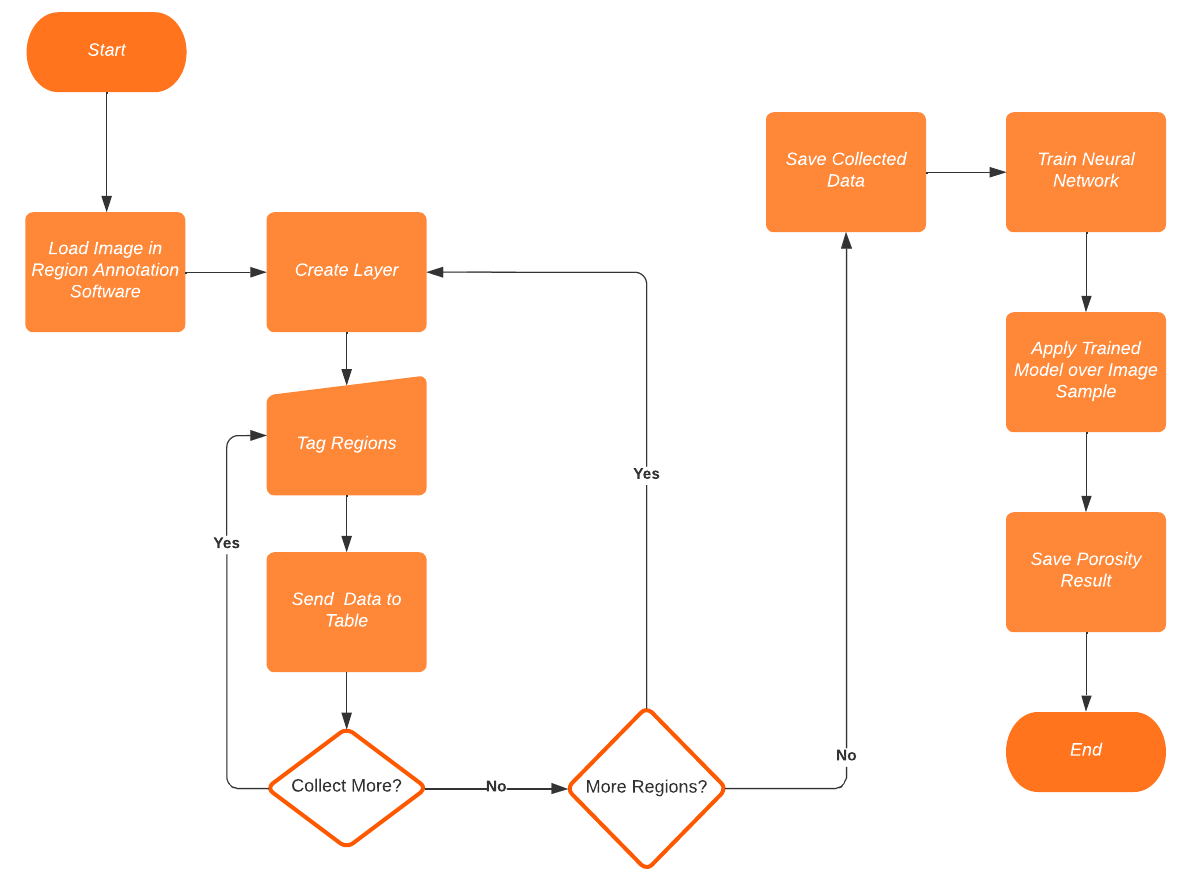
\includegraphics[width=1\textwidth]{images/process}
\par\end{centering}
\caption{Process Overview.\label{fig:process}}
\end{figure}


\subsection{Annotating Regions of Interest Software}

A tool was developed that was capable of displaying an image to the
user, and allowing the regions of interest to be associated with labels
created by the professional who would be using it to carry out the
study on the sample, it would be very useful to obtain material for
feed the AI algorithms. The image to be studied would be loaded onto
a base layer and as new labels were added new layers would overlap
the base layer. The user could then, with some virtual annotation
tool, such as a \textquotedblleft pen\textquotedblright , mark the
regions of interest in each layer. The RGB values of each pixel included
in these marked regions can then be exported to a text file and used
as a dataset in a neural network training script. This idea proved
to be very simple to implement, in addition to having the potential
to collect data for image segmentation of any nature. The Fig. \ref{fig:gui-tool}
shows the tool Graphical User Interface (GUI).

\begin{figure}[H]
\begin{centering}
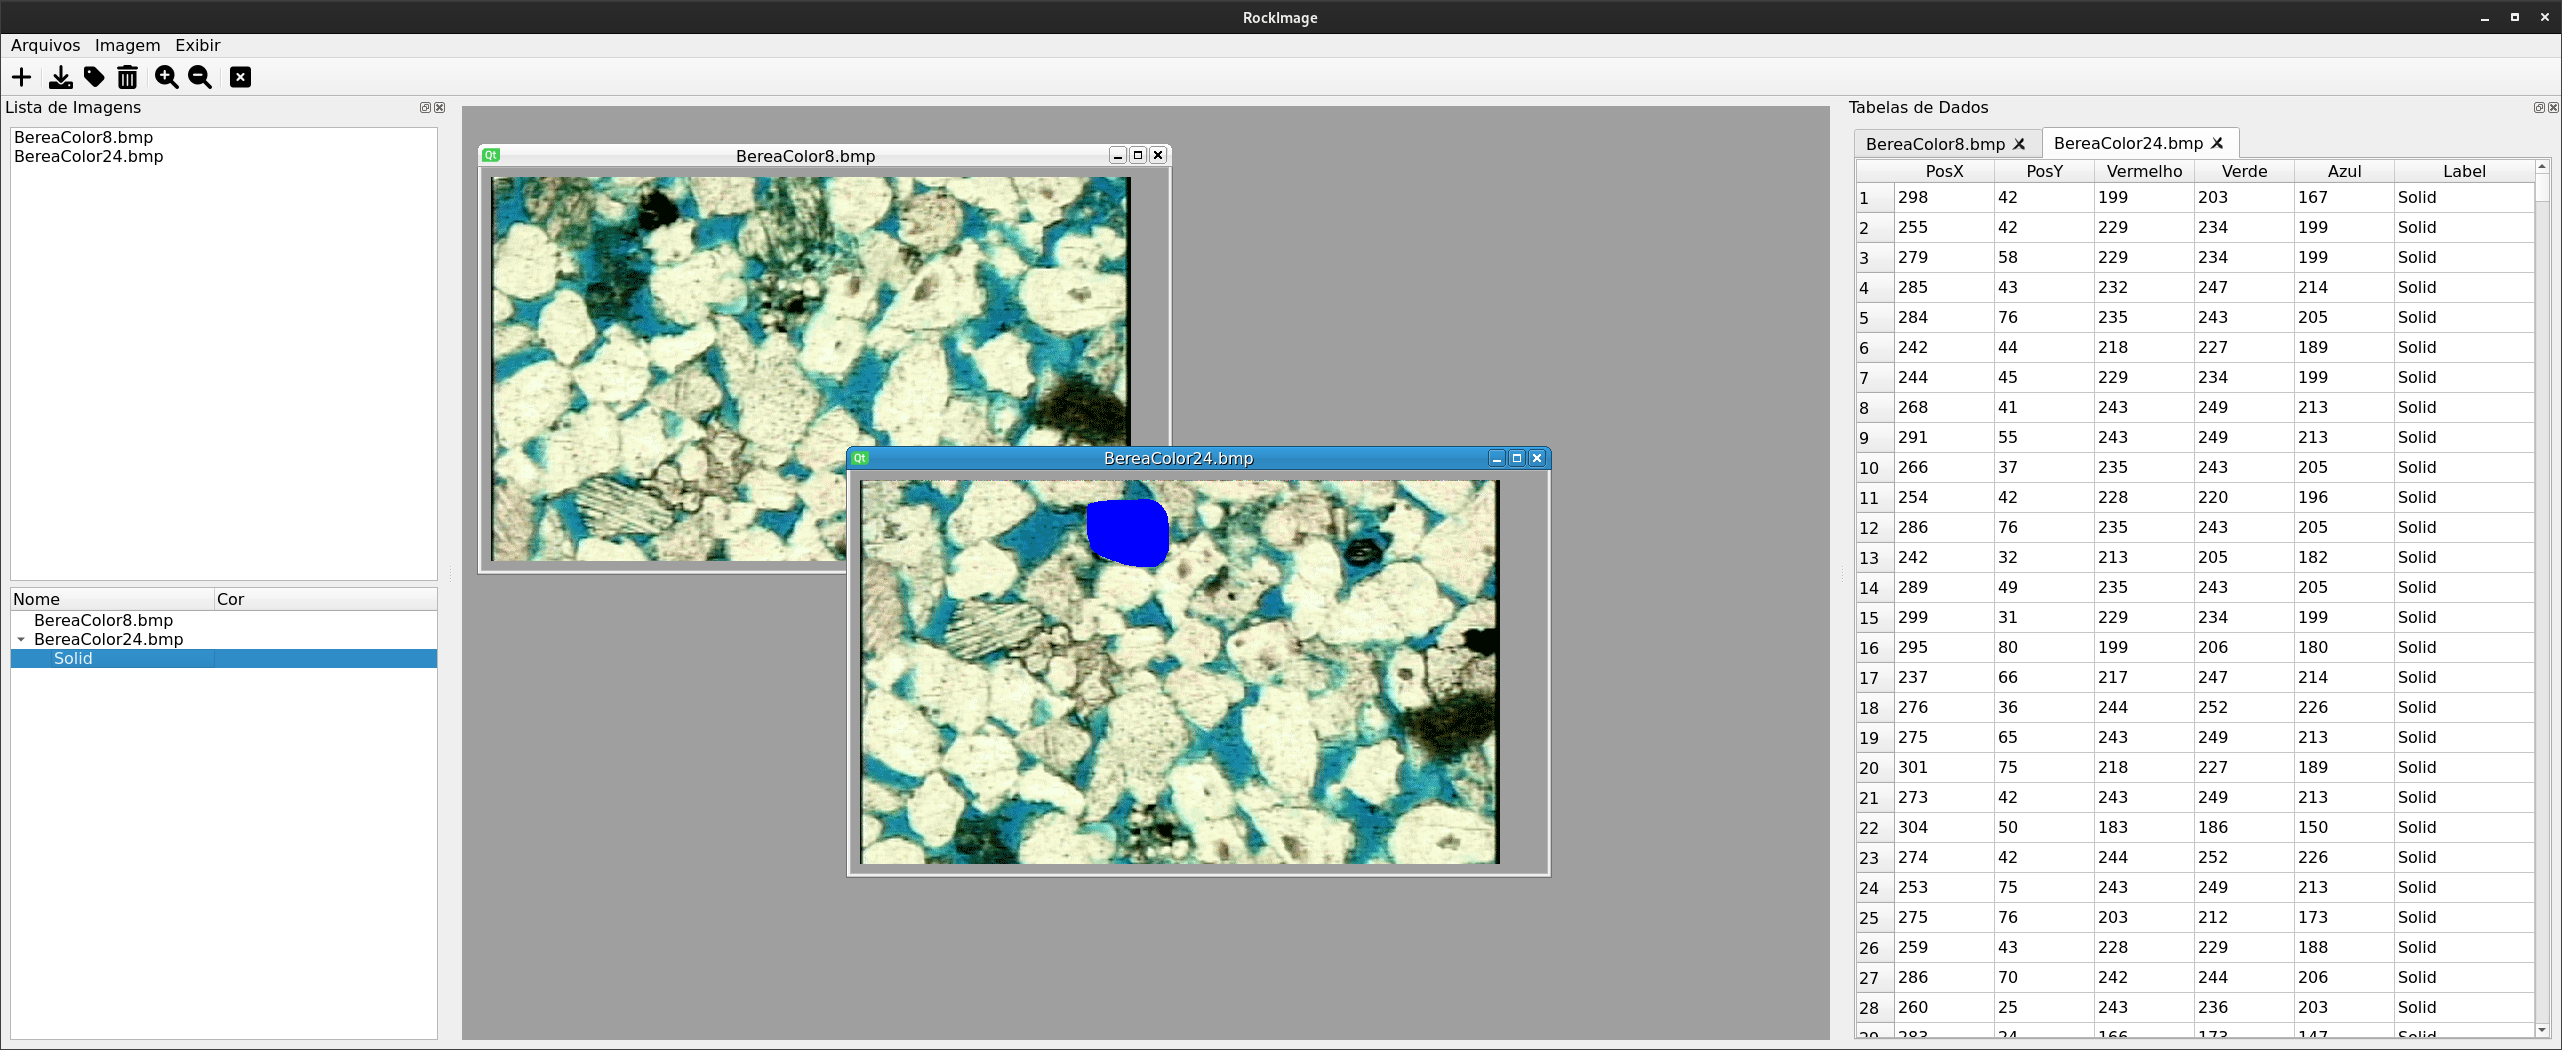
\includegraphics[width=1\textwidth]{images/tool-gui}
\par\end{centering}
\caption{Annotation Tool GUI.\label{fig:gui-tool}}
\end{figure}


\subsection{Data Collecting Process}

The images used for data collection were classified into 5 different
categories, as shown in Table {[}tab:Categories-of-Images{]}, together
with the estimated values of porosity and permeability in $mD$. These
images represent rock samples of different porosity and permeability
values, which implies different ways of performing the collection.
However, actions such as avoiding contact with the edges were taken
to obtain the best data quality.

\begin{table}[H]
\caption{Images Categories.\label{tab:images-categories}}

\noindent \centering{}%
\begin{tabular}{|c|c|c|}
\hline 
Category & Porosity (\%) & Permeability ($mD$)\tabularnewline
\hline 
Berea200 &  & \tabularnewline
\hline 
Berea500 &  & \tabularnewline
\hline 
P148\_K2 & 14,8 & 2\tabularnewline
\hline 
P240\_K104 & 24,0 & 104\tabularnewline
\hline 
P262\_K441 & 26,2 & 441\tabularnewline
\hline 
\end{tabular}
\end{table}

In Figs. \ref{fig:exemple-berea200}, \ref{fig:exemple-berea500},
\ref{fig:exemple-P148_K2}, \ref{fig:exemple-P240_K104}, \ref{fig:exemple-P262_K441}
it is possible to observe an example of data collection using the
tool described above for each image type. During the collection, we
also tried to maintain the same number of points for the regions of
solids and pores. This was done so that it was possible to prevent
the neural network from having its parameters biased during training.

\begin{figure}[H]
\begin{centering}
\subfloat[Berea200 Sample.\label{fig:exemple-berea200}]{\begin{centering}
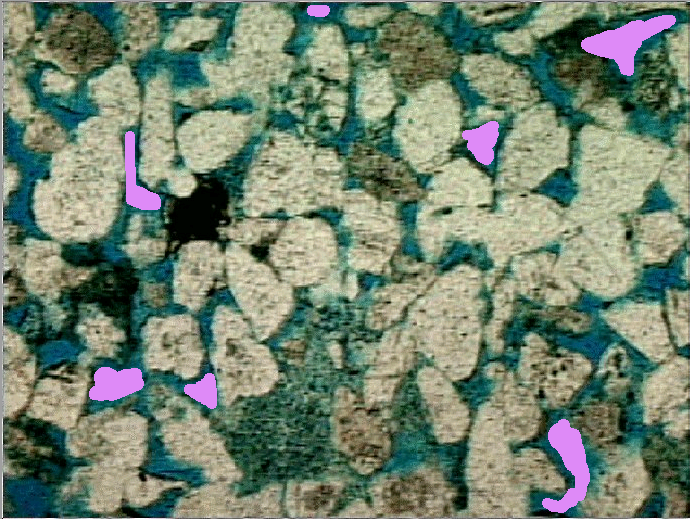
\includegraphics[width=0.32\textwidth]{images/exemplo-i26}
\par\end{centering}
}\subfloat[Berea500 Sample.\label{fig:exemple-berea500}]{\begin{centering}
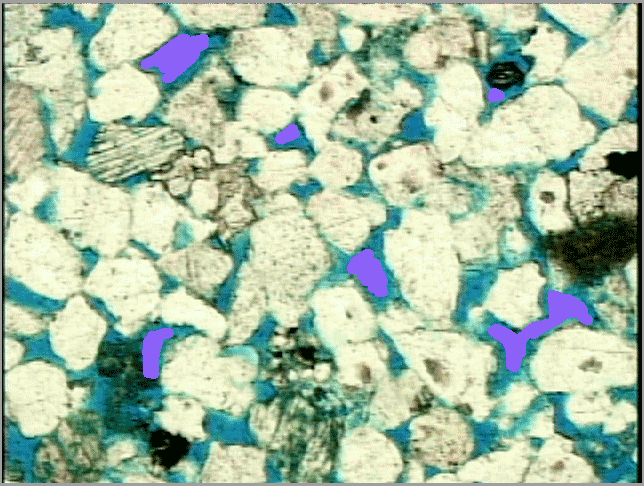
\includegraphics[width=0.32\textwidth]{images/exemplo-berea500}
\par\end{centering}
}\subfloat[P148\_K2 Sample.\label{fig:exemple-P148_K2}]{\begin{centering}
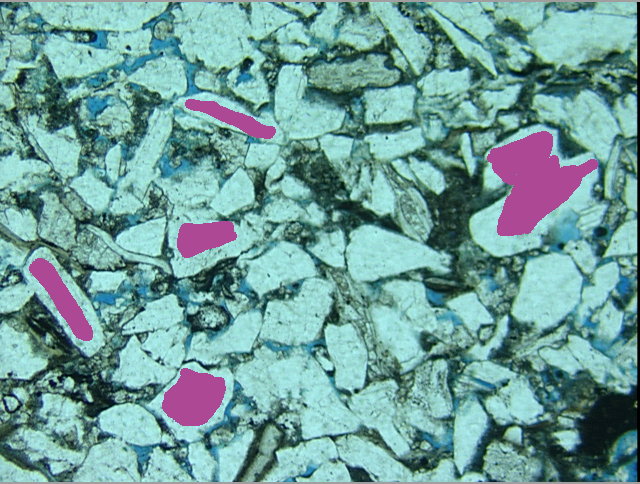
\includegraphics[width=0.32\textwidth]{images/exemplo-p140}
\par\end{centering}
}
\par\end{centering}
\begin{centering}
\subfloat[P240\_K104 Sample.\label{fig:exemple-P240_K104}]{\begin{centering}
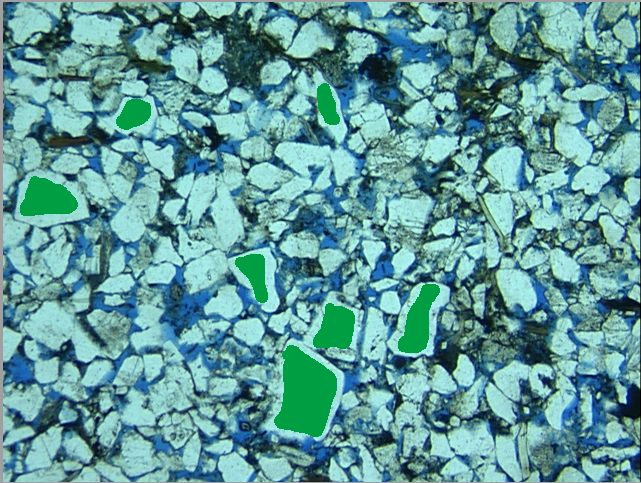
\includegraphics[width=0.32\textwidth]{images/exemplo-p240}
\par\end{centering}
}\subfloat[P262\_K441 Sample.\label{fig:exemple-P262_K441}]{\begin{centering}
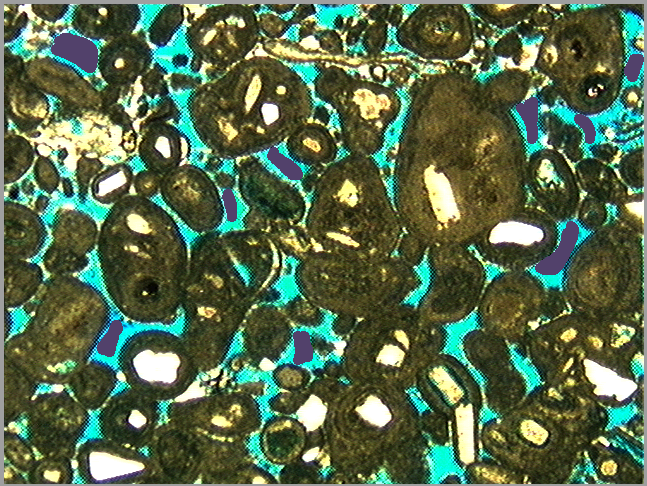
\includegraphics[width=0.32\textwidth]{images/exemplo-p262}
\par\end{centering}
}
\par\end{centering}
\caption{Data Collecting Examples. \label{fig:examples}}
\end{figure}


\subsection{Neural Network Training and Application Process}

\subsubsection{Model Description}

Table \ref{tab:Neural-Networks-Layers} describes the neural network
model used for training and binarizing the images. All internal layers
of this network used ReLU as an activation function. A function called
log\_softmax was used to output the neural network, which, according
to the library documentation, is recommended for classifier algorithms.

\begin{table}[H]
\caption{Neural Networks Layers.\label{tab:Neural-Networks-Layers}}

\noindent \centering{}%
\begin{tabular}{|c|c|c|}
\hline 
Layer Number & Number of Neurons & Activation Function\tabularnewline
\hline 
1 & 4 & \emph{relu}\tabularnewline
\hline 
2 & 4 & \emph{relu}\tabularnewline
\hline 
3 & 4 & \emph{relu}\tabularnewline
\hline 
4 (\emph{output}) & 2 & \emph{log\_softmax}\tabularnewline
\hline 
\end{tabular}
\end{table}

The training process took place for each of the datasets used in the
same way. First, they were loaded through the command line interface
developed in python. Then they are shuffled and divided into training
and test sets. After that, the training set was applied to the neural
network in the form of mini batches. At the end of this step, the
set test was submitted to the neural network to verify the accuracy.
This process was then repeated for 5 epochs for each of the datasets.

\subsubsection{Model Application}

To apply the model, the CLI receives the path to the file that stores
the model saved in pickle, in the training process, the path to the
image that will be binarized, the path to the output binarized image
and a flag to indicate whether the result of the binarized image should
be saved or not.

Once the function is started, an instance of the neural network is
created and the saved model is loaded into it. Then, the image is
transformed into a PyTorch tensor and used to feed the AI model. The
result of this event is the binararized image and the time elapesed.
The porosity of the sample image is then calculated and saved in a
text file.

\section{Results}

In this section, the results obtained from the application of artificial
intelligence methods over digital rocks samples will be shown along
with the segmented images.

\subsection{Porosity Values}

This section presents the results obtained by applying the methods
described in the previous chapter. The Table \ref{tab:porosity-results}
shows the values obtained for porosity in each of the images and the
time elapsed for application of the model.

\begin{table}[H]
\caption{Porosity Results.\label{tab:porosity-results}}

\noindent \centering{}%
\begin{tabular}{|c|c|c|}
\hline 
Sample & Porosity (\%) & Elapsed Time (ms)\tabularnewline
\hline 
\hline 
Berea200 & 25,5654 & 10,3312\tabularnewline
\hline 
Berea500 & 14,4561 & 9,9576\tabularnewline
\hline 
P148\_K2 & 24,5020 & 10,2811 \tabularnewline
\hline 
P240\_K104 & 27,6058 & 22,7351\tabularnewline
\hline 
P262\_K441 & 20,1338 & 9,2697\tabularnewline
\hline 
\end{tabular}
\end{table}


\subsection{Output Images}

The Figs. \ref{fig:exemple-berea200-1}, \ref{fig:exemple-berea500-1},
\ref{fig:exemple-P148_K2-1}, \ref{fig:exemple-P240_K104-1}, \ref{fig:exemple-P262_K441-1}
shows the output images from the binarization process.

\begin{figure}[H]
\begin{centering}
\subfloat[Berea200 Sample.\label{fig:exemple-berea200-1}]{\begin{centering}
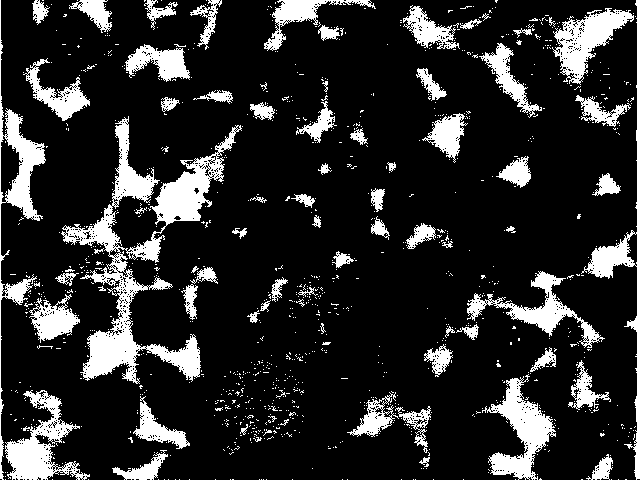
\includegraphics[width=0.32\textwidth]{images/I26-bin}
\par\end{centering}
}\subfloat[Berea500 Sample.\label{fig:exemple-berea500-1}]{\begin{centering}
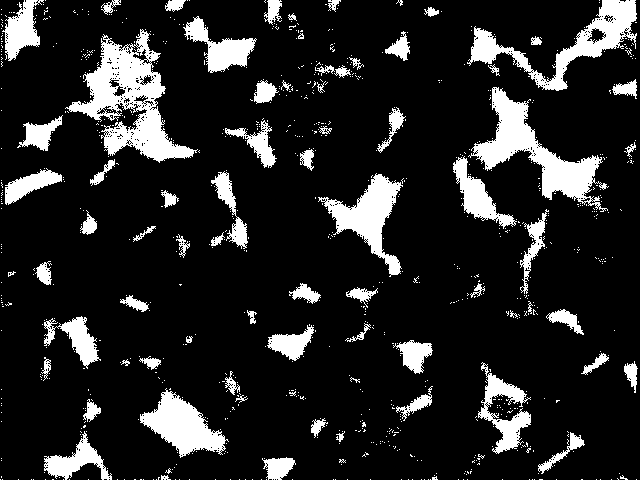
\includegraphics[width=0.32\textwidth]{images/I320-bin}
\par\end{centering}
}\subfloat[P148\_K2 Sample.\label{fig:exemple-P148_K2-1}]{\begin{centering}
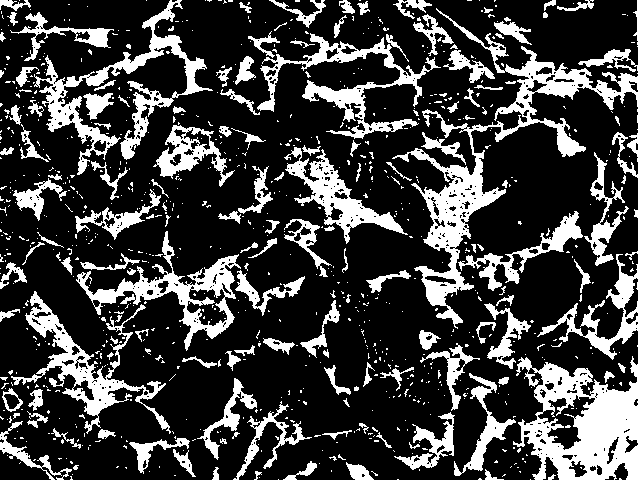
\includegraphics[width=0.32\textwidth]{images/3271i01-bin}
\par\end{centering}
}
\par\end{centering}
\begin{centering}
\subfloat[P240\_K104 Sample.\label{fig:exemple-P240_K104-1}]{\begin{centering}
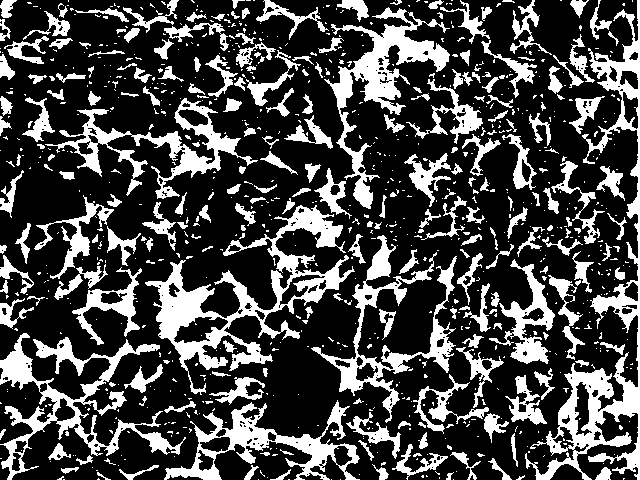
\includegraphics[width=0.32\textwidth]{images/3251i01-bin}
\par\end{centering}
}\subfloat[P262\_K441 Sample.\label{fig:exemple-P262_K441-1}]{\begin{centering}
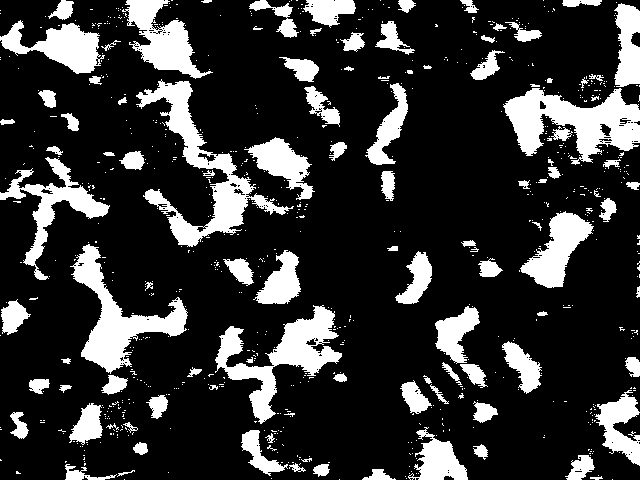
\includegraphics[width=0.32\textwidth]{images/L67409i1-bin}
\par\end{centering}
}
\par\end{centering}
\caption{Output images from binarization process. \label{fig:outputs}}
\end{figure}


\section{Discussion}

As discussed earlier, the use of neural networks to solve problems
related to image segmentation proves to be quite useful, especially
when it comes to the study of digital rock samples. The results shown
above corroborate those already shown in other works, such as \citet{rego2010desenvolvimento,sudakov2019driving,lin2016efficient,leu2014fast,kuroda2016tecnicas,ma2017image}.

What can be highlighted from the porosity values obtained is that
there is a margin of error between the values obtained in the laboratory
and those calculated by the algorithm. This may be related to the
fact that in the laboratory part of the porosity value can be lost
depending on the quality of the equipment used, while its electronic
counterpart is capable of capturing the minutiae in the pores of smaller
radius.

Another point to be considered is the impact that the quality of the
images has on the segmented output. Figs. \ref{fig:exemple-berea200-1},
\ref{fig:exemple-berea500-1} and \ref{fig:exemple-P262_K441-1} have
a result with a much lower visual quality compared to \ref{fig:exemple-P148_K2-1}
and \ref{fig:exemple-P240_K104-1} images.

Finally, the \ref{fig:exemple-P148_K2-1} image has an error in the
porosity value that can be justified by some regions that can be confused
with oil stains, but which in reality can just be an error in the
application of the resin. Figs. \ref{fig:exemple-region-bin} and
\ref{fig:example-image} highlights this region.

\begin{figure}[H]
\begin{centering}
\subfloat[P148\_K2 Sample Output.\label{fig:exemple-region-bin}]{\begin{centering}
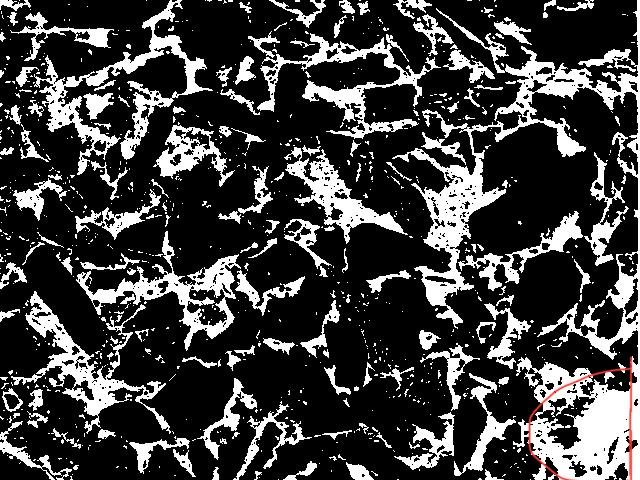
\includegraphics[width=0.32\textwidth]{images/region-bin.jpeg}
\par\end{centering}
}\subfloat[P148\_K2 Sample.\label{fig:example-image}]{\begin{centering}
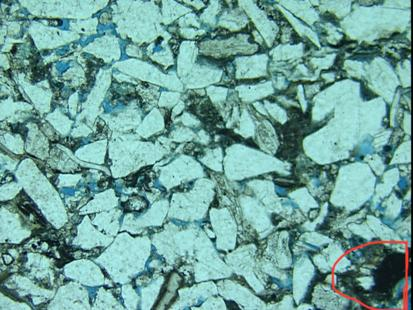
\includegraphics[width=0.32\textwidth]{images/region.jpeg}
\par\end{centering}
}
\par\end{centering}
\caption{Data Collecting Examples. \label{fig:region}}
\end{figure}


\section{Conclusion}

As previously explained, the use of artificial intelligence algorithms
is increasingly common in the most different areas of research, especially
in the field of engineering. The use of such technology makes the
execution of complex tasks, such as the classification and prediction
model, in a short time possible.

More specifically in the field of reservoir engineering, the use of
neural networks and computer vision allow analyzes to be performed
to describe petrophysical characteristics of a sample without having
to damage it. In this work, it was shown how absolute porosity values
can be obtained using intelligent models that allow the segmentation
of images in regions of pores and solid matrix, in a relatively shorter
time and with precision similar to physical analysis. In addition,
the development of these models took place using open source technologies,
which makes it easier to reproduce the results described here.

The general objective of this work was to develop artificial intelligence
methods capable of recognizing relevant patterns for the analysis
of petrophysical properties in images of reservoir rocks. We tried
to study different methods of machine learning and deep learning applied
to image analysis, and to develop applications that could make possible
the application of these models in real world examples. Among these
applications would be python scripts for the use of artificial intelligence
techniques and a tool for annotating regions of interest in digital
rock samples.

Obtaining the results so that the objectives described above were
achieved took place in the form of a procedure described in Figure
\ref{fig:process}, where the color information of the pixels of the
regions of interest were collected and saved in a file in .dat format.
This file is used as inputs for a neural network developed using the
Machine Learning library PyTorch. The training script output is another
file in .pt format, which contains the values of the biases and weights
of the trained neural network. This saved template is then applied
over the image to be binarized. Finally, the porosity value for the
new image generated in the process is calculated. This entire procedure
was repeated for images contained in the digital collection of Prof.
DSc. Andr� Duarte Bueno.

For this work, a single feed-forward neural network model was developed,
with 3 deep layers, each with 4 neurons, as shown in Table \ref{tab:Neural-Networks-Layers}.
As activation function, the ReLU function shown in Equation \ref{eq:relu-func}
was used. For the last layer, the softmax function was applied followed
by the application of the natural logarithm of the value obtained.
As optimizer, the Adam algorithm was chosen and, finally, the loss
function NLL Loss, or, Negative Log-Likelihood Loss.

As a result, the duration of both training and application of the
model lasted in the order of milliseconds, which shows the ability
of these algorithms to deliver results quickly.

This work shows how technologies such as machine learning can be very
useful in obtaining porosity values in samples of reservoir rocks.
Additionally, the use of annotation tools can help make the data collection
process less tedious and tedious.

\bibliographystyle{elsarticle-harv}
\addcontentsline{toc}{section}{\refname}\bibliography{bibliografia}

\end{document}
